\chapter{Project Plan}\label{ch:plan}

\section{Methodology and Approach}
This thesis can be broken down into five major components and milestones.
The first of which is the literature review, as outlined in Chapter~\ref{ch:lit_review}, and the project preparations and viability study, as outlined in Chapter~\ref{ch:project_prep}.
After having reviewed existing exploration into this field, an Ubuntu machine was set up using Open Robotics' Robot Operating System (ROS).
Using the Microsoft Kinect depth sensor in conjunction with ROS, some preliminary tests were run to determine if external devices could reasonably be controlled by reading data from the Kinect.
This produced promising results and hence this setup will be used to run the smart home automation, as shown in Figure~\ref{fig:simple_tech_stack}.

\begin{figure}[!htb]
    \caption{Simplified Technology Stack}
    \centering
    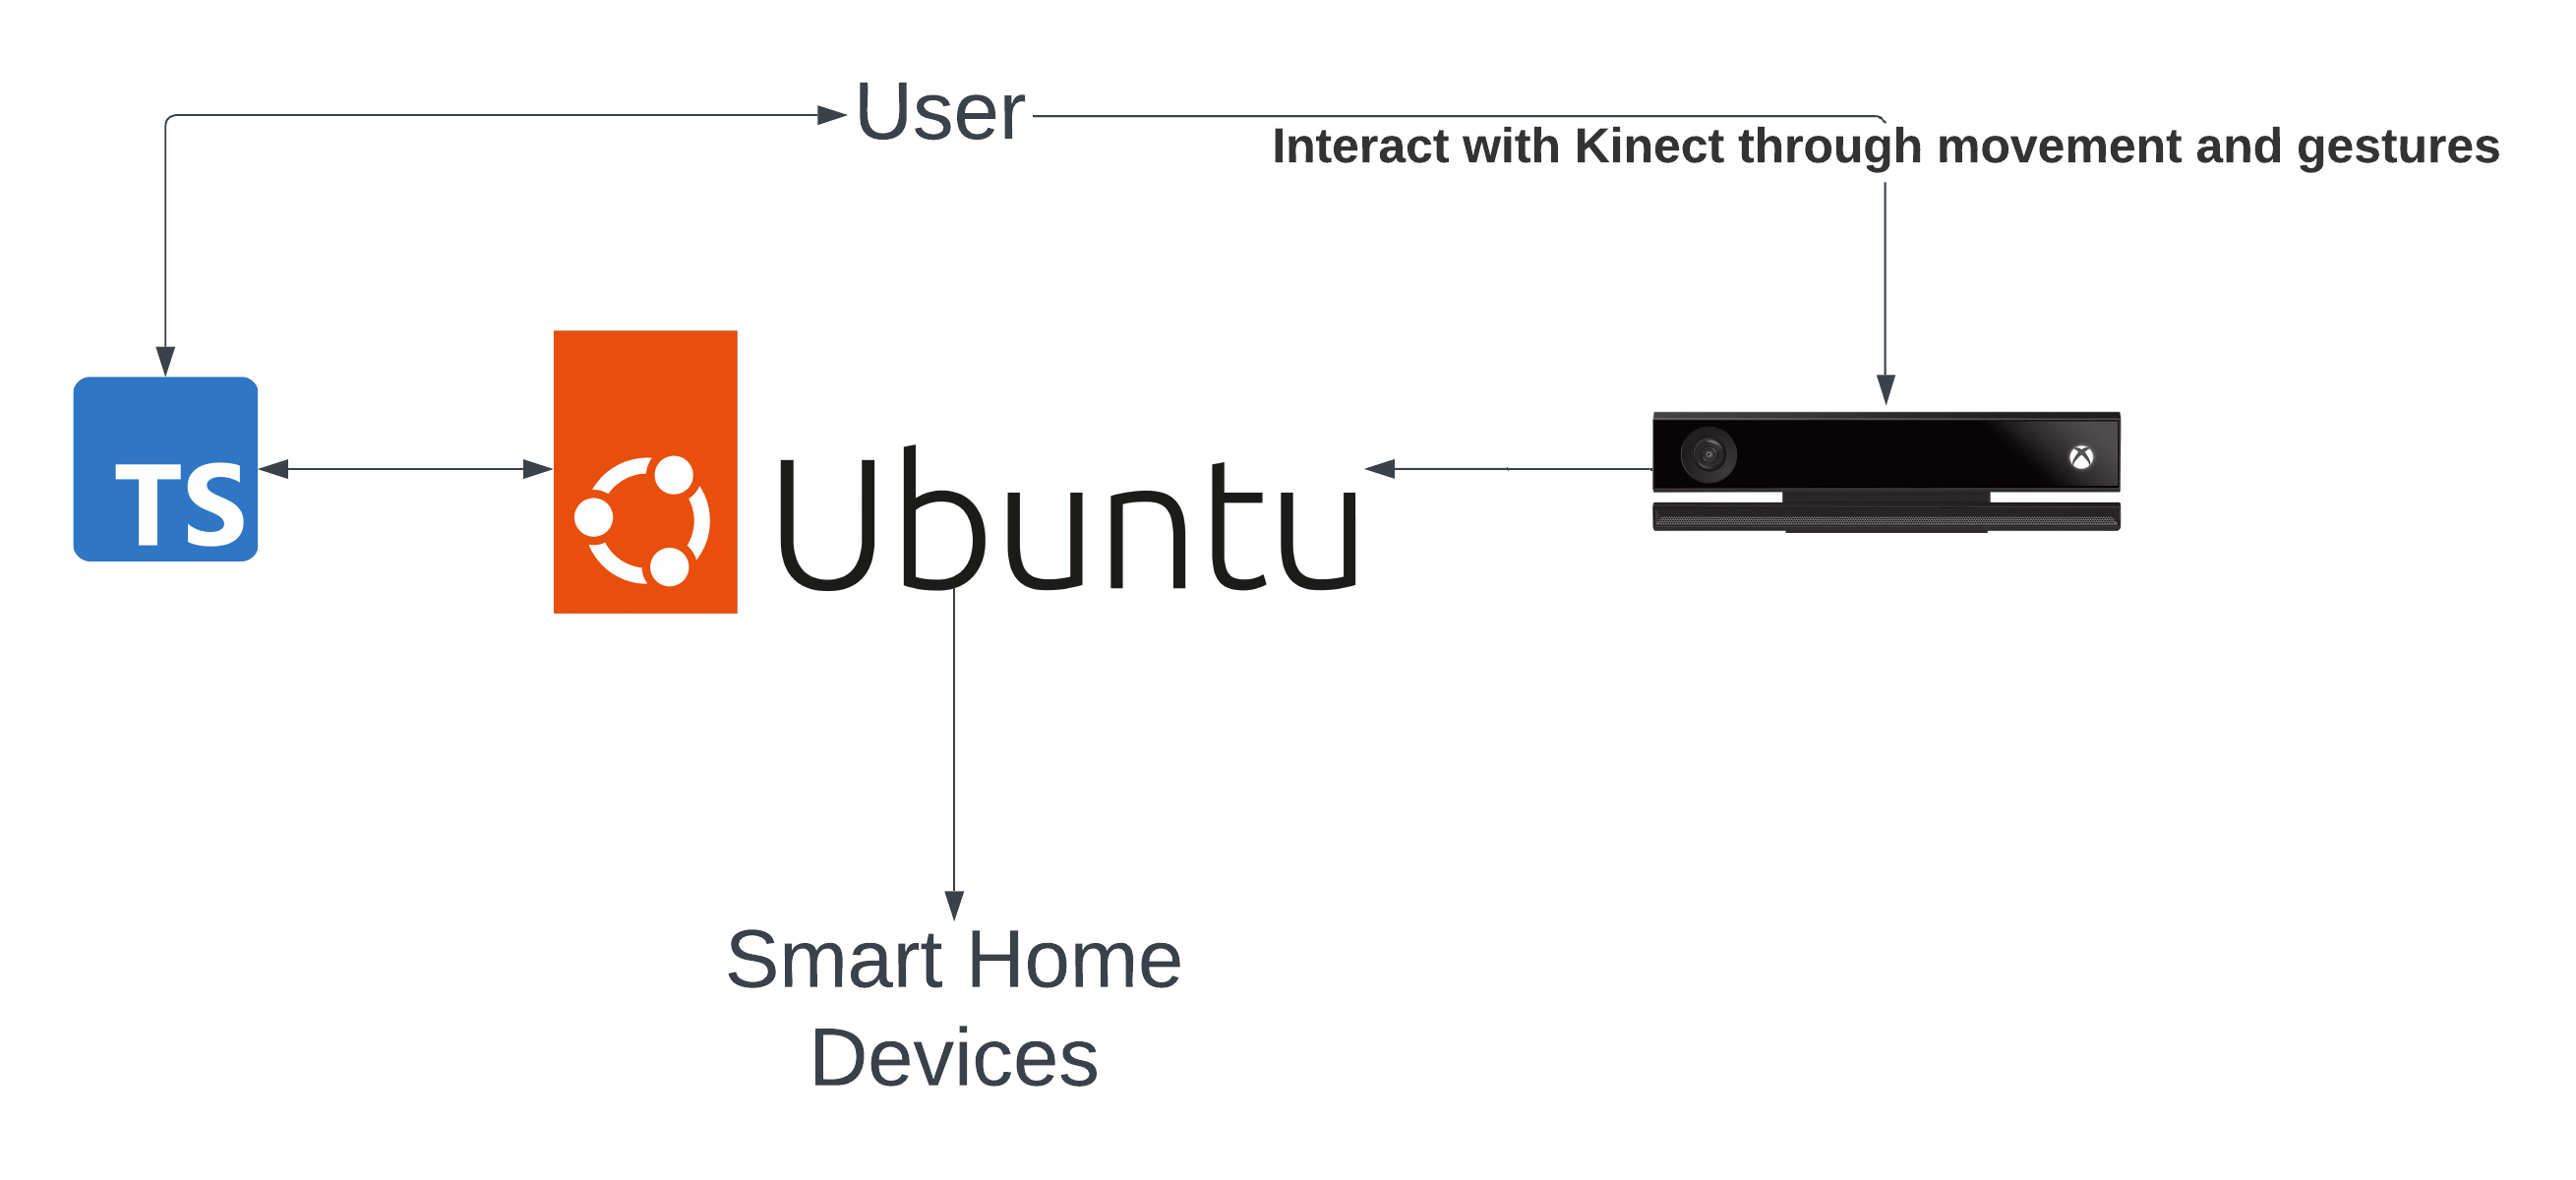
\includegraphics[width=\textwidth]{Simplified Tech Stack.png}
    \label{fig:simple_tech_stack}
\end{figure}

Following this, in the coming months, the project will be broken down into the following main goals:

\begin{itemize}
    \item Implement Yolo v8
    \item Train AI model
    \item Create web interface
    \item Evaluate performance
\end{itemize}

The first goal is to implement Yolo v8, a real-time object detection system.
With this, the system will be able to detect users in the environment and track their movements.
With the built-in pose estimation, the system will be able to determine the user's pose and use this information to make predictive decisions based on the user's routine historically and read gestures to make decisions in real time.

Subsequently, the AI model will be trained on a custom data set built from the data collected from the Kinect in the lab environment.
Yolo also has built-in model training which will allow for a simple and efficient training process.
This will mean that the system will be trained on the specific environment and users that it will be deployed in, allowing for a more accurate and efficient system.

The third component of the project is a TypeScript (TS) web interface that allows users to control devices manually and customise and add new gestures.
This is because the smart home system should only ever add functionality to a home, never replace existing functionality, so users should have the option to control the devices manually.

Finally, the performance of the system will be evaluated.
There are five metrics that will determine the success of the project deployment:
\begin{itemize}
    \item Rate of false positives
    \item Rate of false negatives
    \item Rate of true positives
    \item Speed of execution, and
    \item Perceived increase in convenience
\end{itemize}

The first four are measurable quantitative metrics, while the fifth adds a qualitative aspect to the evaluation, taking into consideration how real users perceive the system.
This will be conducted through user testing.

\subsection{Stretch Goals}
If these goals are met earlier in the timeline than expected, there have been stretch goals in consideration that could be pursued.
For a real smart home deployment, it would be more realistic and convenient for users if the computer running the system was much smaller than the laptop that is currently in use.
A Raspberry Pi is capable of running an Ubuntu distro and running the required software while significantly smaller and could be tucked away into a cupboard.
This has not been entirely explored yet and it may not be feasible due to the depth data processing that is somewhat computationally intensive.

Another consideration that has been made is using multi-modal input to control devices.
Implementing a system that can control devices through multiple methods could provide a more seamless user experience and allow for more flexibility in how users interact with their devices.
Using gestures and voice commands in conjunction could allow users to control devices with more natural behaviours, for example, turning on a light by saying ``turn the lights on'' and then making a gesture to indicate which light they want to turn on.
This could also allow for integration with existing robots used in the lab, giving them an instruction via voice and pointing to a location or object, indicating where or what they should perform that action on.

\section{Timeline}

\begin{figure}[!htb]
    \caption{Project Timeline}
    \centering
    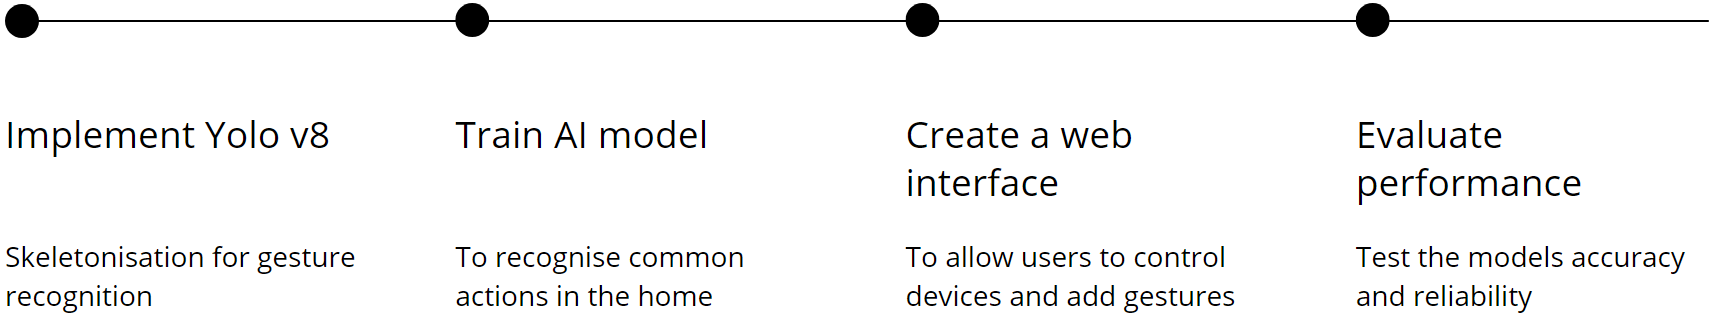
\includegraphics[width=\textwidth]{Timeline.png}
    \label{fig:timeline}
\end{figure}

It is expected that each of the main stages of the project, as shown in Figure~\ref{fig:timeline}, will on average take approximately two weeks to complete and have a thorough implementation working.
This is a rough estimate and some stages may take longer or shorter than expected.

Implementing Yolo may be the fastest stage, perhaps achievable in one week, as it is a well-documented and widely used system, while training the AI model may take longer as it is dependent on the quality of the data collected and the performance of the system.
The web interface should in theory be a straightforward process but will take time to achieve a polished and user-friendly interface.
Evaluating the performance should also be relatively simple but it will take time to collect the data and analyse it, and this would be the period where any problems could arise, delaying progress.

\begin{description}
    \item[Implement Yolo v8] 1-2 weeks
    \item[Train AI Model] 2-3 weeks
    \item[Create web interface] 2 weeks
    \item[Evaluate performance] 1-2 weeks    
\end{description}

This accounts for approximately eight weeks of work, leaving two weeks at the end of the term as a buffer in case of any unexpected delays, as well as time to prepare for a demonstration and the final presentation.

\section{Required Training and Upskilling}
There are a few areas that will require some upskilling to complete this project, including learning how to use ROS, Yolo, and TypeScript.

ROS tools can be controlled through the command line, and many of their tutorials teach you how to use these to control devices and virtual robots like the turtle simulator.
These tutorials are great for learning how ROS nodes, services, and topics work, and how to send messages using these to control devices.
ROS messages can also be sent via Python or C++ code, using the ROS client libraries, which will be useful for writing the programs to control devices in the home so both of these will be necessary to learn for the project.

Using the ROS client library for Python will also allow for the use of the Yolo v8 implementation, as it is written in Python.
Yolo, fortunately, has extensive documentation, so using their software should be relatively easy to learn, though the concepts that are used in object detection and pose estimation will need to be understood to use the software effectively.

AI and Machine Learning are not new concepts, having taken COMP3411 - Artificial Intelligence.
However, this course covers the concepts of AI and ML, not the practical implementation of these concepts.
Using ML to train an AI model will require some significant upskilling to complete in practice.

Another area that will require some upskilling is the use of IoT devices.
Sending state change signals to devices uses similar underlying principles to other known concepts such as web development but the exact implementation with IoT devices will require some learning.

Finally, the web interface will be built using TypeScript, a superset of JavaScript (JS) that adds static typing to the language.
JavaScript is an already known language so the move to TS is not a significant leap, but using typing in JS is a new skill that will need to be learned and adapted to.